\chapter{Математическая модель движения мобильных плавающих роботов}\label{ch:ch2}

\section{Описание математчиеской модели движения мобильного робота в форме эллипсоида в жидкости}\label{sec:ch2/sec1}

Движение произвольного тела в жидкости в предположении, что вязкие эффекты отсутствуют, описывается уравнениями Кирхгофа \cite{Kirchhoff}

\begin{gather}
\frac{d}{dt}\left( \der{T}{\bV} \right) = \der{T}{\bV} \times \bOm,\quad \frac{d}{dt} \left(\der{T}{\bOm}\right) = \der{T}{\bOm} \times \bOm + \der{T}{\bV} \times \bV,\label{eq.Kirchhoff}
\end{gather}
где $T$ -- кинетическая энергия системы (оболочка + жидкость + роторы), $\bV$ и $\bOm$ -- скорость центра оболочки и его угловая скорость.

Суммарная кинетическая энергия тела имеет вид
\begin{gather}
T_s = \frac{1}{2} m_s \left( \bV,\, \bV \right) + \frac{1}{2} \left( \bOm,\, \bbI_s \bOm \right),
\end{gather}
где $m_s$ -- масса оболочки, $\bbI_s$ -- главный центральный тензор инерции оболочки.

Кинетическая энергия жидкости
\begin{gather}
T_f = \frac{1}{2} \left( \bV,\, \bLam _V \bV \right) + \left( \bV,\, \bbB \bOm \right) + \frac{1}{2} \left( \bOm,\, \bLam_\Omega \bOm \right),
\end{gather}
где $\bLam_V = \diag (\lambda_{1},\, \lambda_{2},\, \lambda_{3})$ -- тензор присоединенных масс, $\bLam_\Omega = \diag (\lambda_{4},\, \lambda_{5},\, \lambda_{6})$ -- тензор присоединенных моментов инерции, $\bbB = \diag (b_{1},\, b_{2},\, b_{3})$ -- тензор, возникающий вследствие винтовой симметрии тела. Диагональный вид тензоров $\bLam_V$, $\bLam_\Omega$ и $\bbB$ связан с наличием центральной симметрии у оболочки, отсутствием смещения центра масс относительно геометрического центра тела и выбором системы координат таким образом, что одна из координатных осей совпадает с ось симметрии тела. Вообще говоря, для тела, показанного на рис. \ref{constr_BPR}, тензоры $\bLam_V$, $\bLam_\Omega$ и $\bbB$ будут иметь по два равных коэффициента $\lambda_1 = \lambda_2$, $\lambda_4 = \lambda_5$, $b_1 = b_2$. Однако, все дальнейшие рассуждения без потери общности будут проводиться для несимметричного случая.

Согласно \cite{Korotkin} при соответствующем выборе системы координат для двухлопастного винта тензоры $\bLam_V$, $\bLam_\Omega$ и $\bbB$ будут симметричными. Для четырехлопастного винта $\bLam_V$ и $\bLam_\Omega$ будут диагональными, а $\bbB$ -- симметричным. Для винта с пятью и более лопастями $\bLam_V$, $\bLam_\Omega$ и $\bbB$ будут диагональными.

Кинетическая энергия $k$-го ротора определяется выражением
\begin{gather}
T_k = \frac{1}{2} m_k \left( \bV,\, \bV \right) + \frac{1}{2} \bigl( \bOm + \omega_k(t) \bn_k,\, \bbI_k \left( \bOm + \omega_k(t) \bn_k \right) \bigr),
\end{gather}
где $m_k$ -- масса ротора $k$-го ротора, $\bbI_k$ -- центральный тензор инерции $k$-го ротора, $\bn_k$ -- единичный вектор, задающий направление оси вращения $k$-го ротора, $\omega_k(t)$ -- угловая скорость вращения $k$-го ротора.

Так как вектор $\bn_k$ является собственным для матрицы $\bbI_k$, то выполняется соотношение $\bbI_k \bn_k = j_k \bn_k$, где $j_k$ -- момент инерции $k$-го ротора относительно оси вращения. С учетом этого суммарная кинетическая энергия системы с точностью до известной функции времени имеет вид

\begin{gather}
T = T_s + T_f + \sum_{k=1}^{3} T_k = \frac{1}{2} \left( \bV,\, \bbC \bV \right) + \left( \bV,\, \bbB \bOm \right) + \frac{1}{2} \left( \bOm,\, \bbI \bOm \right) + \left( \bOm,\, \bK(t) \right), \label{eq.T}
\end{gather}
где $T_s$ -- кинетическая энергия оболочки, $T_f$ -- кинетическая энергия жидкости, $T_k$ -- кинетическая энергия $k$-го ротора; $\displaystyle \bK(t) = \sum_{k=1}^{3} j_k \omega_k(t) \bn_k$ -- вектор гиростатического момента, $\bbB = \diag (b_{1},\, b_{2},\, b_{3})$ -- тензор, возникающий вследствие винтовой симметрии тела. Матрицы $\bbC$ и $\bbI$ имеют вид
\begin{gather}
\begin{gathered}
\bbC = m \bbE + \bLam_V = \diag (c_1,\, c_2,\, c_3),\quad m = m_s + 3 m_k,\\
\bbI =\bLam_\Omega + \bbI_s + \sum_{k=1}^{3} \bbI_k = \diag (i_1,\, i_2,\, i_3).
\end{gathered}
\end{gather}
где $m_s$ -- масса оболочки, $\bbI_s$ -- главный центральный тензор инерции оболочки, $\bLam_V = \diag (\lambda_{1},\, \lambda_{2},\, \lambda_{3})$ -- тензор присоединенных масс, $\bLam_\Omega = \diag (\lambda_{4},\, \lambda_{5},\, \lambda_{6})$ -- тензор присоединенных моментов инерции, , $m_k$ -- масса ротора $k$-го ротора, $\bbI_k$ -- центральный тензор инерции $k$-го ротора, $\bn_k$ -- единичный вектор, задающий направление оси вращения $k$-го ротора, $\omega_k(t)$ -- угловая скорость вращения $k$-го ротора

Подставив \eqref{eq.T} в уравнения \eqref{eq.Kirchhoff} и, обозначив импульс системы и ее кинетический момент как
\begin{gather}
\bp = \bbC \bV + \bbB \bOm, \quad \bM = \bbB \bV + \bbI \bOm + \bK(t),\label{eq.pMexpr}
\end{gather}
получим уравнения движения в виде
\begin{gather}
\begin{gathered}
\dot{\bp} = \bp \times \bOm , \quad
\dot{\bM} = \bM \times \bOm + \bp \times \bV,
\end{gathered}\label{eq.pM}
\end{gather}

Решение системы дифференциальных уравнений (\ref{eq.pM}) позволит найти положение робота в пространстве и его ориентацию, при заданном векторе внутреннего гиростатического момента $\bK$.


\section{Описание математчиеской модели движения недеформируемого рыбоподобного робота в жидкости}\label{sec:ch2/sec2}

\section{Схема управления мобильными водоплавающими роботами}\label{sec:ch2/sec3}

В полученных математических моделях управление роторами задается в виде вектора внутреннего гиростатического момента $\bK$. Для управления отдельным двигателем разработана следующая схема (см. рисунок \ref{Control_system}).

\begin{figure}[h]
	\centering
	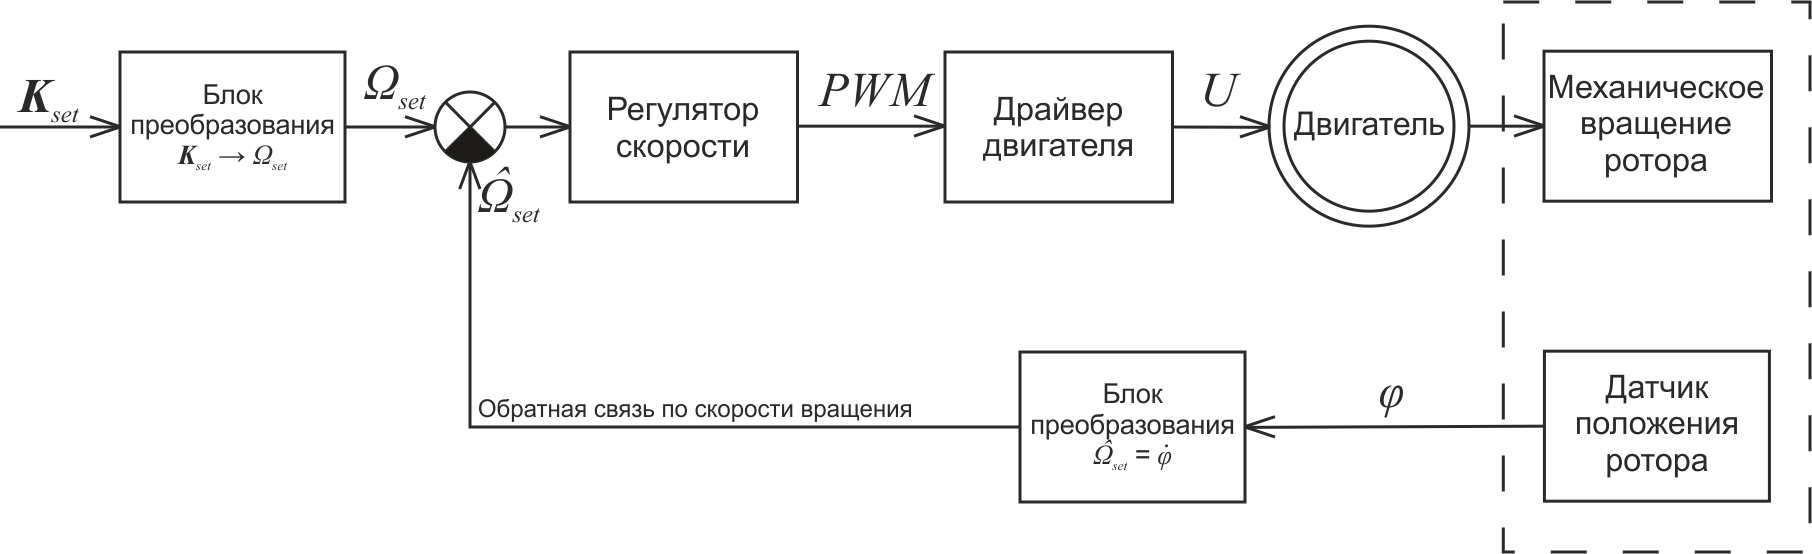
\includegraphics[width=0.9\linewidth]{Control_system.png}%
	\caption{Схема управления отдельным двигателем, где $\bK_{set}$ -- вектор внутреннего гиростатического момента; $\bOm_{set}$ -- угловая скорость вращения двигателя; $\hat{\bOm}_{set}$ -- фактическая скорость вращения двигателя; $PWM$ -- широтно-импульсная модуляция, рассчитаная для заданной скорости вращения; $U$ -- напряжение, подаваемое на двигатель; $\varphi$ -- фактическое положение ротора}
	\label{Control_system}
\end{figure}
